\section{Data and Parameters}
\label{sec:data_and_parameters}

The model is described by a large number of parameters that govern the number of contacts
a person has, the reduction in contacts due to NPIs, the demand for rapid tests and PCR
tests, the likelihood of becoming infected on each contact, the likelihood of developing
light or strong symptoms or even dying from the disease as well as the duration each
stage of the disease takes.

\subsection{Course of the Disease}
\label{sub:course_of_disease}

The following medical parameters describing the progression of the disease are taken from systematic reviews (e.g. \citet{He2020}). After an infection occurs, the disease progresses in the way depicted in Figure~\ref{fig:course_of_disease}.

\begin{figure}[!tp]
    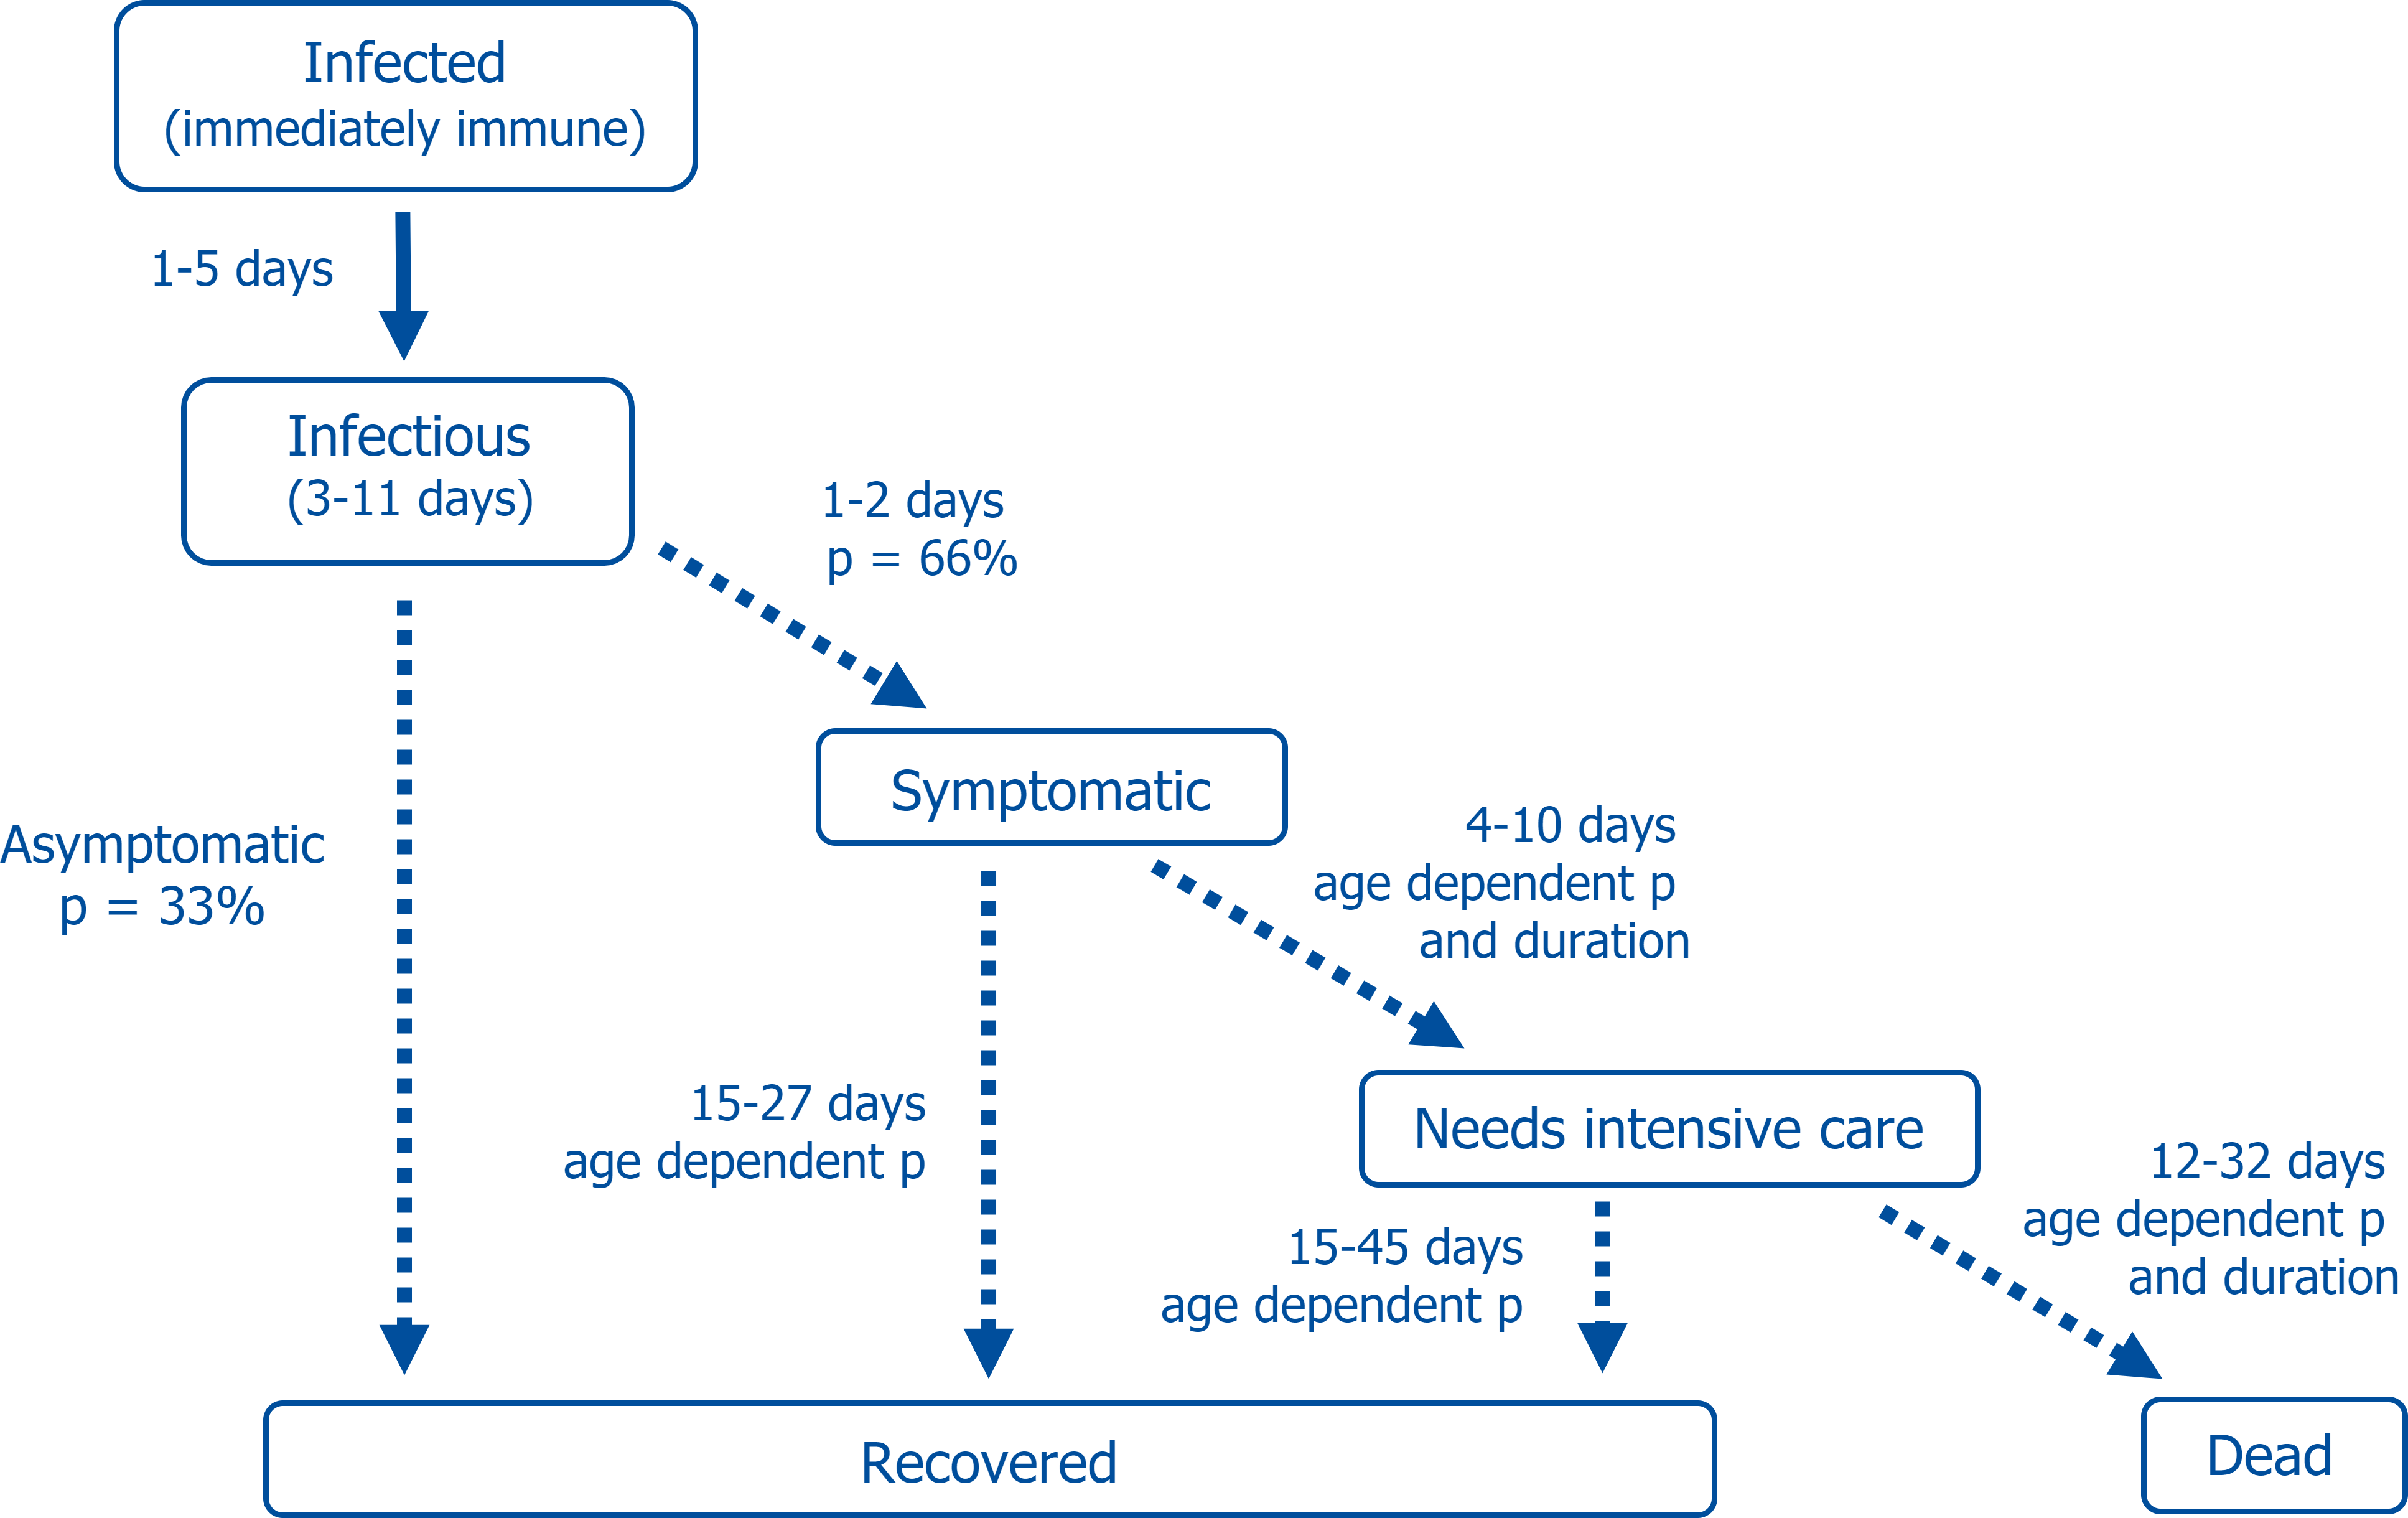
\includegraphics[width=\textwidth]{../figures/disease_progression.png}
    \caption{Course of Disease in the model}
    \label{fig:course_of_disease}
\end{figure}

First, infected individuals will become infectious after one to five days. About one third of people stays asymptomatic. The rest develops symptoms about one to two days after they become infectious. Modeling asymptomatic and pre-symptomatic cases is important because those people do not reduce their contacts or demand a test and can potentially infect many other people \citep{Donsimoni2020}.

A small share of symptomatic people will develop strong symptoms that require intensive care. The exact share and time span is age-dependent. An age-dependent share of intensive care unit (ICU) patients will die after spending up to 32 days in intensive care. Moreover, if the ICU capacity was reached, all patients who require intensive care but do not receive it die.

It would be easy to make the course of disease even more fine-grained. For example, we could model people who require hospitalization but not intensive care. So far we opted against that because only the ICU capacity might become a bottleneck in Germany.

We allow the progression of the disease to be stochastic in two ways: Firstly, state changes only occur with a certain probability (e.g. only a fraction of infected individuals develops symptoms). Secondly, the number of periods for which an individual remains in a state is drawn randomly. The parameters that govern these processes are taken from the literature. They can vary with the age of an individual.

Detailed information on the calibration of the disease parameters is available as part of our \href{https://sid-dev.readthedocs.io/en/latest/reference_guides/epi_params.html}{online documentation}.


\subsection{The Synthetic Population}
\label{subsec:synthetic_population}

We build a synthetic population based on the German microcensus \citep{FDSAeDBUDL2018}.
We only use private households, i.e. exclude living arrangements such as nursing homes as
non-private households vary widely in size and it is very difficult to know which
contacts take place in such living arrangements.

We sample households to build our synthetic population of over one million households
keeping for each of the 2.3 million individuals their age, gender, occupation and whether
they work on Saturdays and Sundays. For each household we draw its county and set the
corresponding federal state.% we draw the county because county is not part of the campus file

We randomly assign 35\% of children below three to attend a nursery \citep{Destatis2020}.
For children between three and six years old, we assume all go to preschool (officially
92.5\% according to \cite{Destatis2020}).
% nurseries and preschools
Children that attend a nursery meet in groups of four \citep{BertelsmannStiftung2019}
plus one adult care taker every weekday when there are no school vacations. Preschool
children meet in groups of nine \citep{BertelsmannStiftung2019} with two adult care
takers. These groups are mixed with respect to age but all belong to the same state and
mostly to the same county.

% school
Every child that goes to school is part of a school class. Each school class meets
three times per weekday, each time with a different set of two teachers, unless
there are vacations or policies that suspend schools.\footnote{We
implement vacations on the federal state level.} Each class consists of approximately 23
students \citep{OECD2013}. All students in a class are of the same age
and live in the same state and mostly also in the same county. In addition, each
child gets assigned a value that captures his or her need to attend nursery, preschool or
school. This allows us to capture various degrees of emergency care that can be granted
while educational facilities are closed or are on some kind of rotating schedule.

% workers
Workers are assigned to a daily meeting work group. The group sizes vary to match the
number of daily repeating work contacts reported by working individuals in
\cite{Mossong2008}. These groups only consist of workers that work in the same county.
For a distribution of the number of daily recurring work contacts see
Figure~\ref{fig:n_contacts_work_daily_recurrent}. To match the number of weekly work groups
we match each worker with up to 14 other workers into pairs to match the number of
reported weekly work contacts shown in Figure~\ref{fig:n_contacts_work_weekly_recurrent}.
Each pair is assigned a weekday on which they always meet in the absence of work
policies. 80\% of these contacts are individuals from the same county.
% work contact priority
In the same way children have an educational priority determining if they are entitled to
emergency care workers are assigned a work contact priority that captures how necessary
their work is and to which degree they can work from home. This means that it's always
the same individuals that continue to have work contacts when work from home mandates of
a certain strictness are in place.

% other recurring contacts
In addition to creating groups for educational facilities and work we also have other
recurring contacts to represent things like groups of friends or sports teams that
practice regularly together. Both daily and weekly groups are created analogously to the
work groups but matching the numbers in Figure~\ref{fig:n_contacts_other_daily_recurrent}
and Figure~\ref{fig:n_contacts_other_weekly_recurrent}. In addition, since leisure
contacts are highly assortative by age all individuals that have a daily leisure contact
are matched with a person not only from the same county but also from the same age group.

% individual responses
The individuals in our population can react to events such as developing symptoms that
are typical of CoViD-19, a positive PCR test or a positive rapid test by reducing their
contacts. To determine who would reduce their contacts in such a situation or demand a
rapid test we introduce a quarantine compliance parameter. Similarly, we introduce a
rapid test compliance parameter that determines in which order individuals start
demanding rapid tests when rapid tests become increasingly available. This makes sure
that when for example only 10\% of workers get tested, it's the same workers that have
access to tests every week.

% vaccination rank
Lastly, for the distribution of vaccinations every individual is assigned a vaccination
group and a vaccination rank from that group that creates a complete vaccination queue
over the population including a share that refuses to be vaccinated ($\xi$) which we
calibrate to  15\% \citep{RKI2021c}. The vaccination groups are created to match the
recommendations by the Ständige Impfkommission \citep{VygenBonnet2020}.\footnote{We cover
that teachers were prioritized more than recommended by the commission.} To cover that
the Pfizer-BioNTech vaccine was later approved for younger age groups we put adolescents
and children into two groups that follow after the general population. These groups do
not become eligible within our simulation frame until June. The way vaccinations are
rolled out in our model is shown in Figure~\ref{fig:vaccinations_by_age_group}.

\begin{figure}[ht]   % vaccinations by age group
  \centering
  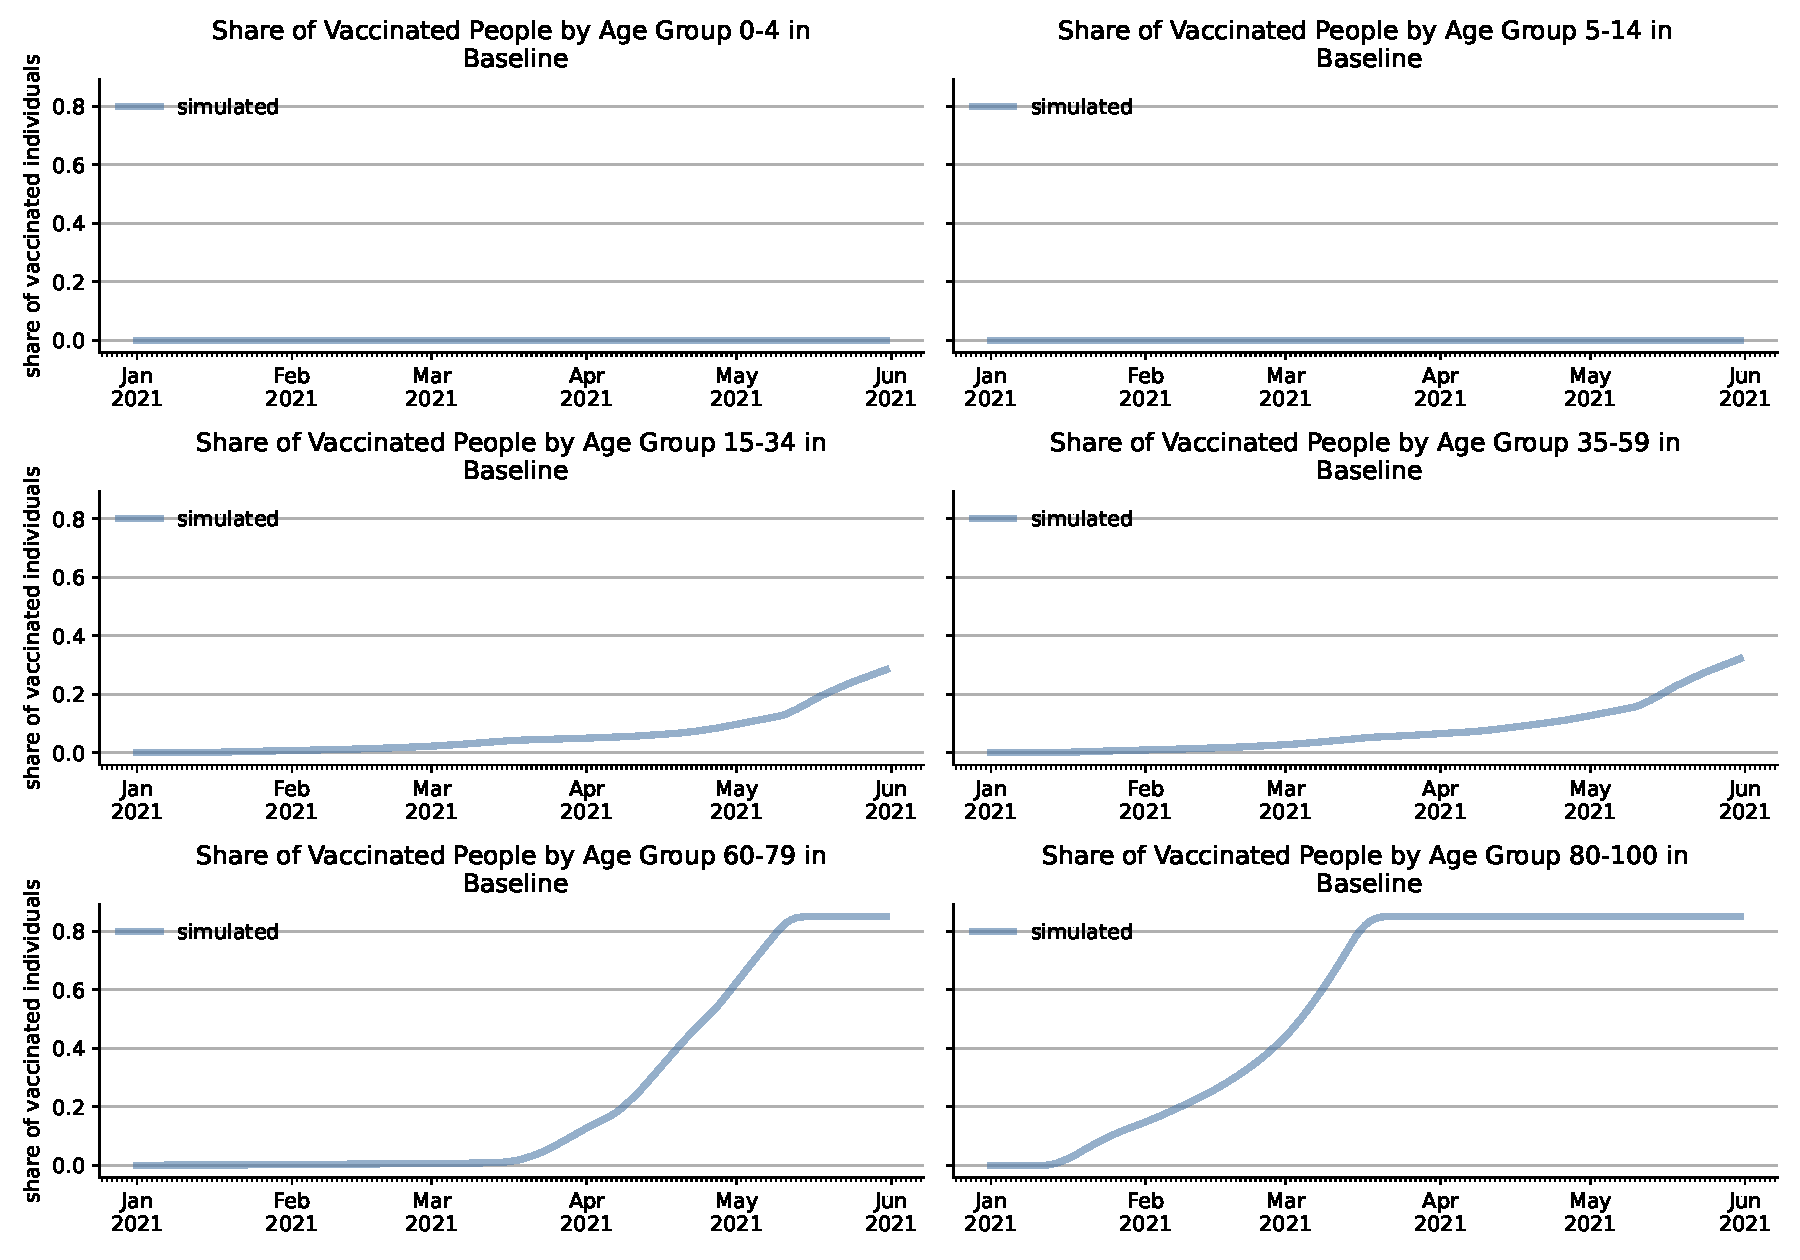
\includegraphics[width=\textwidth]{figures/results/figures/vaccinations/spring_baseline}
  \caption{Vaccination Rates by Age Group}
  \floatfoot{\noindent \textit{Note:} An individual's vaccination priority depends on her
  work contact priority, her age group and a random component to capture
  preconditions like diabetes. 15\% of the population refuse to be vaccinated ($\xi$).
  Adolescents would be vaccinated after the general population and children last. The
  figure clearly shows that the first vaccinations go to some workers with very high work
  contact priority and to the 80 to 100 age group followed by the 60 to 79 year olds.
  Both groups are saturated with vaccinations by mid March and start of May respectively.
  By June a third of the younger adults have received the vaccination but these groups
  still remain far from herd immunity thresholds.}
  \label{fig:vaccinations_by_age_group}
\end{figure}

\FloatBarrier


\subsection{Modeling Numbers of Contacts}
\label{sec:number_of_contacts}

Consider a hypothetical population of 1,000 individuals in which 50 were infected with a
novel infectious disease. From this alone, it is impossible to say whether only
those 50 people had contact with an infectious person and the disease has an infection
probability of 1 per contact or whether everyone met an infectious person but the
disease has an infection probability of only 5 percent per contact. SEIR models do not
distinguish contact frequency from the infectiousness of each contact and
combine the two in one parameter that is not invariant to social distancing policies.

To model social distancing policies, we need to disentangle the effects of the number of
contacts of each individual and the effect of policy-invariant infection probabilities
specific to each contact type. Since not all contacts are equally infectious, we
distinguish different contact types.

The number and type of contacts in our model can be easily extended. Each type of
contacts is described by a function that maps individual characteristics, health states
and the date into a number of planned contacts for each individual. This allows to model
a wide range of contact types.

In our empirical application we distinguish the following  contact types that
are depicted in Figure~\ref{fig:model_contacts_infections} and can be further grouped
in the categories household, work, education and others.

types of contacts:

\begin{itemize}
    \item Households: Each household member meets all other household members every day.
    % Household sizes and structures are calibrated to be representative for Germany.


    \item Recurrent work contacts, capturing contacts with coworkers, repeating
          clients and superiors. Some of these recurrent contacts take place on
          every workday, others just once per week.

    \item Random work contacts: Working adults have contacts with randomly drawn other
          people, which are assortative in geographical location and age.


    \item Schools: Each student meets all of his classmates every day. Class sizes are
    calibrated to be representative for Germany and students have the same age. Schools
    are closed on weekends and during vacations, which vary by states. School classes
    also meet six teachers everyday and some of the teachers meet each other.

    \item Preschools: Children who are at least three years old and younger than six may
    attend preschool. Each group of nine children interacts with the same two adults
    every day. The children in each group are of the same age. The remaining mechanics
    are similar to schools.

    \item Nurseries: Children younger than three years may attend a nursery and interact
    with one adult. The age of the children varies within groups. The remaining
    mechanics are similar to schools.

    \item Random other contacts: Contacts with randomly drawn other
    people, which are assortative with respect to geographic location and and age group.
    This contact type reflects contacts during leisure activities, grocery shopping,
    medical appointments, etc..

    \item Recurrent other contacts representing contacts with friends neighbors or
        family members who do not live in the same household. Some of these contacts
        happen daily, others only once per week.


\end{itemize}

The number of random and recurrent contacts at the workplace, during leisure activities
and at home is calibrated with data provided by \citet{Mossong2008}. For details see
Section~\ref{subsec:data_number_of_contacts}. In particular, we sample the number of
contacts or group sizes from empirical distributions that sometimes depend on age. It
would also be possible to use economic or other behavioral models to predict the number
of contacts.

% Theoretically, each contact type can have its own infection probability. However, to
% reduce the number of free parameters and thus avoid a potential over-fitting we only
% estimate different infection probabilities for the areas work, school, preschool and
% nurseries, households and other contacts.


\subsection{Assortativity}
\label{subsec:assortativity}

As explained in section \ref{sec:matching}, the probability that two individuals are
matched can depend on background characteristics. In particular, we allow this
probability to depend on age and county of residence ($\alpha$). While we do not have
good data on geographical assortativity and set it such that 80\% of contacts are within
the same county, we can calibrate the assortativity by age from \cite{Mossong2008}.

\begin{figure}[ht]
    \centering
    \begin{subfigure}[b]{0.425\textwidth}
        \centering
        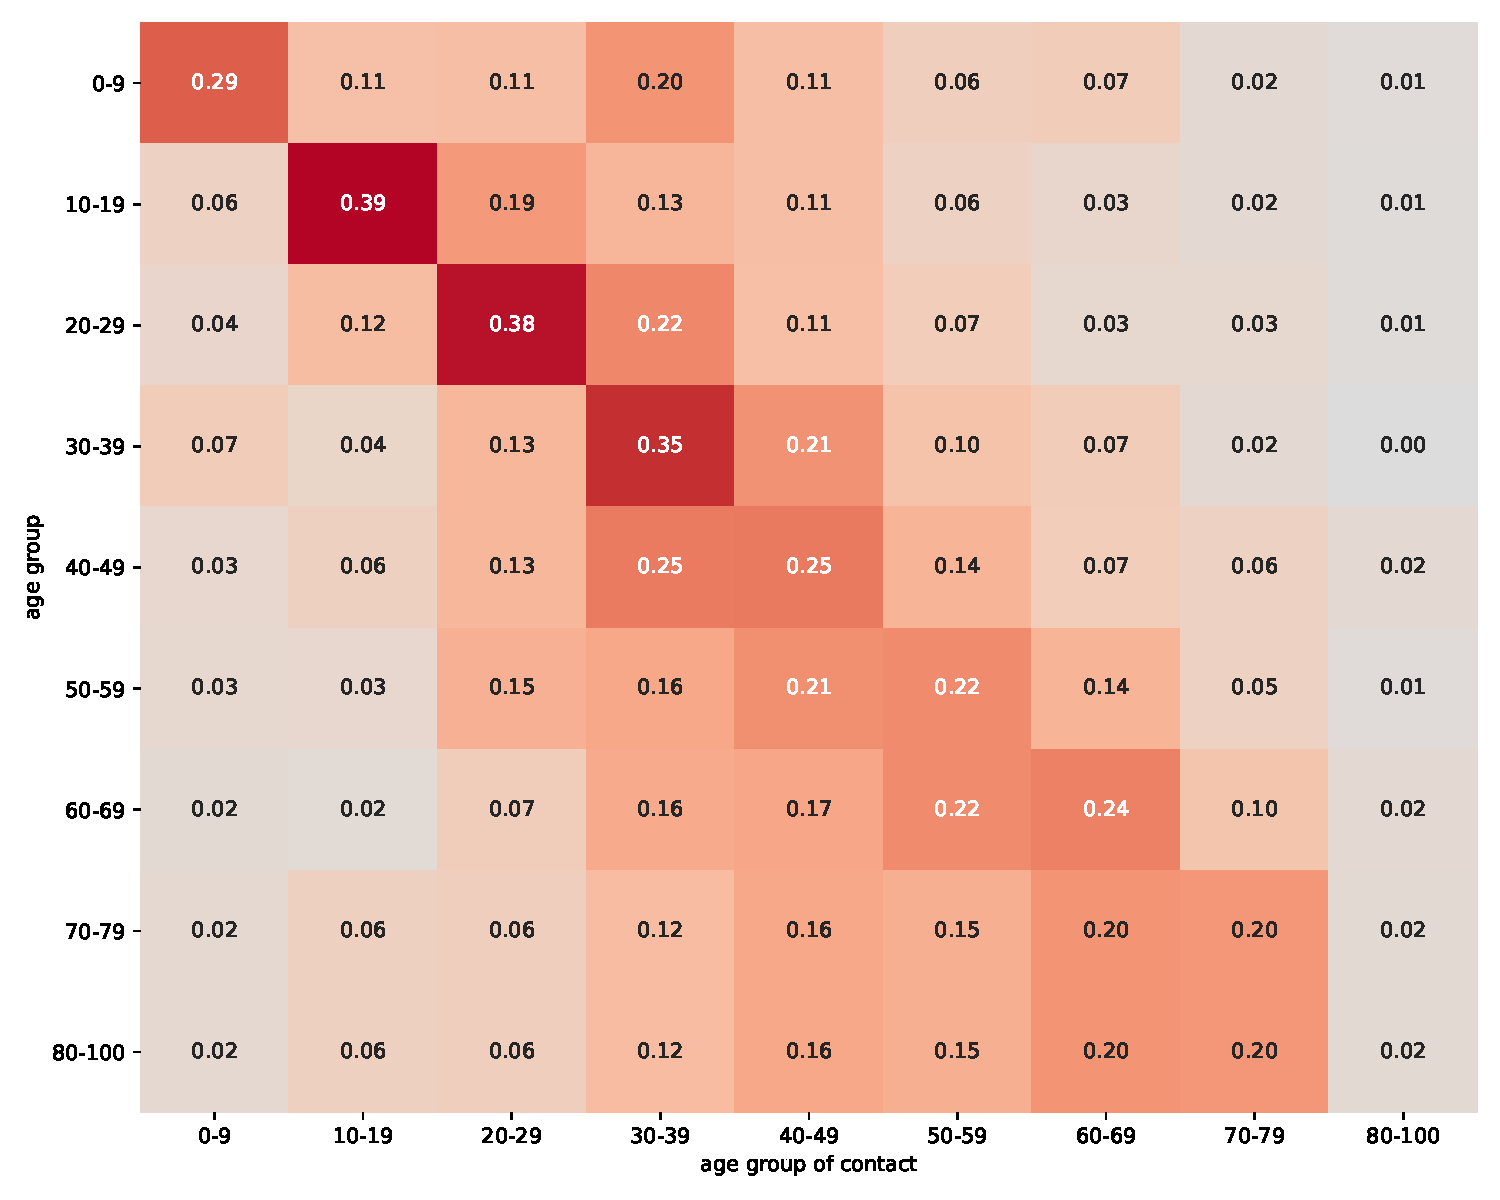
\includegraphics[width=\textwidth]{figures/results/figures/data/assortativity_other_non_recurrent}
        \caption{{Distribution of Non Recurrent Other Contacts by Age Group}}
        \label{fig:assortativity_other}
    \end{subfigure}
    \hfill
    % work assortativity
    \begin{subfigure}[b]{0.425\textwidth}
        \centering
        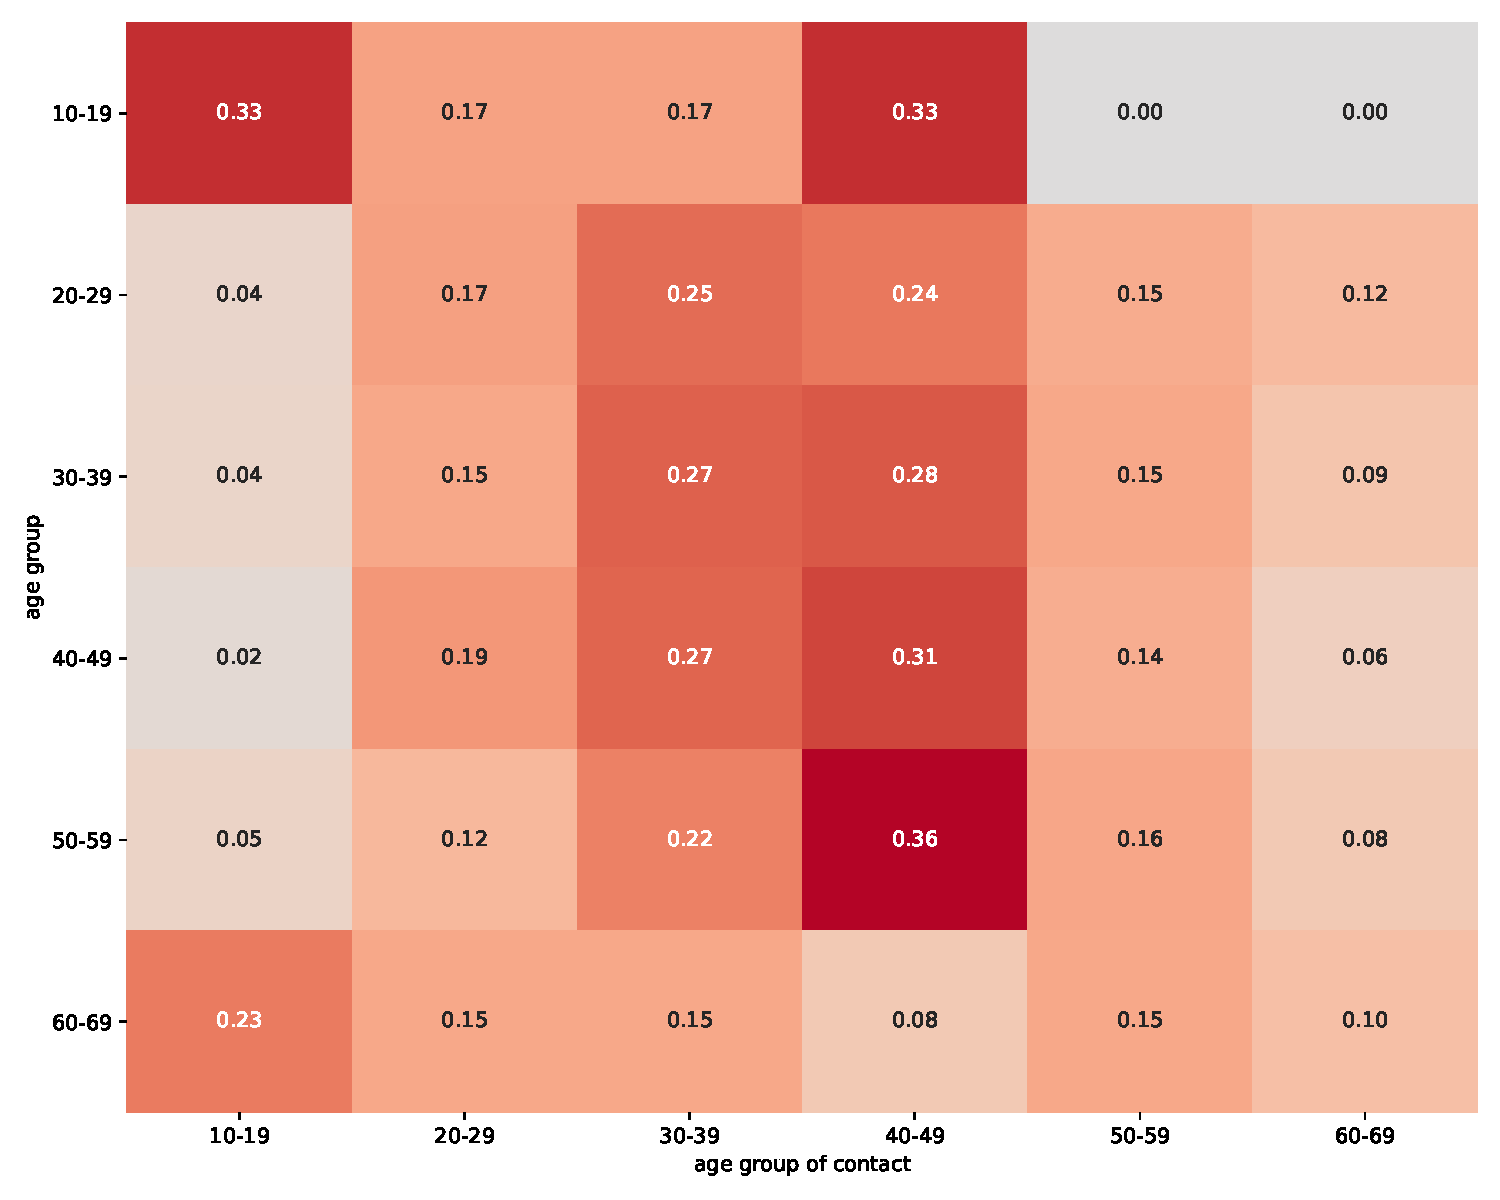
\includegraphics[width=0.9 \textwidth]{figures/results/figures/data/assortativity_work_non_recurrent}
        \caption{{Distribution of Non Recurrent Work Contacts by Age Group}}
        \label{fig:assortativity_work}
    \end{subfigure}

    \vskip3ex


    \caption{Assortativity by Age Group for Non Recurrent Other and Work Contacts}
    \floatfoot{\noindent \textit{Note:} The figure shows the distribution of non
        recurrent contacts by age group for other contacts on the left and work contacts
        on the right. A row shows the share of contacts a certain age group has with all
        other age groups. Higher values are colored in darker red tones. The diagonal
        represents the share of contacts with individuals from the same age group. The
        80-100 age group for other contacts was so small that we assumed for them to have
        the same contact distribution as the 70-79 year olds. For work contacts, we only
        show age groups that have a significant fraction of working individuals.}

    \label{fig:assortativity}

\end{figure}


Figure~\ref{fig:assortativity_other} shows that assortativity of the other contacts by
age is especially strong for children and adolescents. For older people, the pattern
becomes more dispersed around their own age group, but within-age-group contacts are
still the most common contacts. Figure~\ref{fig:assortativity_work} shows that
assortativity by age is also important among work contacts.

For recurrent contacts, we constructed groups to have the following features: Recurrent
work contacts are not assortative by age. Daily work groups are always of the same county
and weekly work contacts are to 80\% with workers from the same county. Other recurrent
contacts are constructed the same way but we impose for daily contacts that they are
always with individuals from the same age group. School classes are groups where the same
children of the mostly same age and county meet with teachers every day. Nurseries and
preschools mix children by age but match them to come mostly from the same county.
Household age composition follows directly from the German microcensus data we use to
construct our synthetic population.

\FloatBarrier

\subsection{Reducing Numbers of Contacts via NPIs}
\label{sec:policies}

Our model makes it very easy to model a wide range of NPIs, either in isolation or
simultaneously. This is important for two reasons: Firstly, it allows to predict and
quantify the effect of novel NPIs. Secondly, it allows to model the actually implemented
policy environment in great detail, which is necessary to use use the full time series
of infections and fatality rates to estimate the model parameters.\footnote{
See \citet{Avery2020} for an explanation why it can be harmful to use too long time
series to estimate simple SEIR type models.}


Instead of thinking of policies as completely replacing how many contacts people have,
it is often more helpful to think of them as adjusting the pre-pandemic number of
contacts. Therefore, we implement policies as a step that happens after the number of contacts is
calculated but before individuals are matched.

On an abstract level, a policy is a functions that modifies the number of contacts of
one contact type. This function can be random or deterministic. For example, school
closures simply set all school contacts to zero. A work from home mandate leads to a
share of workers staying home every day whereas those who cannot work from home are
unaffected. Hygiene measures at work randomly reduce the number of infectious contacts
for all workers who still go to work.

Policies can also interact. For example, school vacations are temporally reducing school
contacts to zero while at the same time increasing other contacts to account for
increased leisure activities and family visits during this time. This is important to
reproduce the finding that school vacations do not reduce infection numbers even though
schools lead to infections when open \citep{Isphording2021}.

The most complex policies are typically found in the education sector. Since the
beginning of 2021 schools have switched back and fourth between full closures,
split class approaches with alternating schedules for some or all age groups and
reopening while maintaining hygiene measures. On top of that there are different
policies for allowing young students whose parents work full time to attend school
even on days where they normally would not. For details on how we calibrate these
policies see Section~\ref{subsec:policies}.

Importantly, policies can depend on the health states of participating individuals.
This allows to quarantine entire school classes if one student tested positive or
to implement official or private contact tracing.

For some policies the exact effect on each contact type is not easy to determine. If
this refers to a policy has been active during the estimation period, it is possible to
estimate such parameters by fitting the model to time series data of infection rates.
This is only possible if the policy was not active during the whole estimation period
and thus the infection probabilities can be identified separately. We do this to account
for hygiene measures at school and in the workplace that have been in effect since
November 2020.

Not all things that reduce contacts compared to the pre-pandemic level are driven
by NPIs. Therefore, we also model endogenous contact reductions that can depend on
the health state of individuals, known risk contacts or the local incidence of
infections. Examples are strong contact reductions for symptomatic individuals or those
who have a positive PCR or rapid tests or contact reductions when a houshold member
tested positive. The extent to which contacts are reduced can be calibrated from
surveys. For an application of our model showcasing private contact tracing in the
context of the Christmas holidays see \cite{Gabler2020}.








\subsection{Rapid Test Demand}
\label{subsec:rapid_test_demand}

In our model, there are five reasons why rapid tests are done:\comment[id=J]{ Add a
    section on how we calibrate rapid test demand; Mainly describe the datapoints we have
    and say that we usually interpolate linearly in between data points. (Only exception
    to that is private rapid test demand, which we fit to data)
}

\begin{enumerate}
    \item someone plans to have work contacts
    \item someone is an employee of an educational facility or a school pupil
    \item a household member has tested positive or developed symptoms
    \item someone has developed symptoms but has not received a PCR test
    \item someone plans to participate in a weekly non-work meeting
\end{enumerate}

%%% \subsubsection{work rapid tests}

For work contacts, we know from the COSMO study (\cite{Betsch2021}, 20th/21st of April)
that 60\% of workers who receive a test offer by their employer regularly use it. We
assume this share to be time constant.

In addition, there are some surveys that allow us to trace the expansion of employers who
offer tests to their employees. Mid march, 20\% of employers offered tests to their
employees \citep{DIHK2021}. In the second half of March, 23\% of employees reported being
offered weekly rapid tests by their employer \citep{Ahlers2021}. This share increased to
61\% until the first days of April \citep{BMWI2021, IZA2021}.

Until mid April 72\% of workers were expected to receive a weekly test offer
\citep{BMWI2021, IZA2021}. However, according to surveys conducted in mid April
\citep{Betsch2021}, less than two thirds of individuals with work contacts receive a test
offer. Starting on April 19th employers were required by law to provide two weekly tests
to their employees \citep{Bundesanzeiger2021}. We assume that compliance is incomplete
and only 80\% of employers actually offer tests.

%%\subsubsection{educ rapid tests}

We assume that employees in educational facilities start getting tested in 2021 and that
by March 1st 30\% of them are tested weekly. The share increases to 90\% for the week
before Easter. At that time both Bavaria \citep{STMGP2021} and Baden-Württemberg
\citep{MinisteriumKultus2021} were offering tests to teachers and North-Rhine Westphalia
\citep{SchulministeriumNRW2021} and Lower Saxony \citep{NSMK2021} were already testing
students and tests for students and teachers were already mandatory in Saxony
\citep{SMK2021}. After Easter we assume that 95\% of teachers get tested twice per week.

Tests for students started later \citep{MinisteriumKultus2021, SchulministeriumNRW2021}
so we assume that they only start in February and only 10\% of students get tested by
March 1st. Relying on the same sources as above we approximate that by the week before
Easter this share had increased to 40\% \citep{SchulministeriumNRW2021}.

After Easter the share of students receiving twice weekly tests is set to 75\%. This is
based on tests becoming mandatory in Bavaria \citep{BayerischeStaatskanzlei2021} and
North Rhine-Westphalia \citep{SchulministeriumNRW2021b} after their Easter breaks and
on the 19th in Baden-Württemberg \citep{KMBaWue2021}.

%%\subsubsection{private rapid tests}

To limit our degrees of freedom, we only have one parameter that governs how many
individuals do a rapid test because of any of the private demand reasons (own symptoms
but no PCR test, planned weekly leisure meeting or a symptomatic or positively tested
household member).

We assume that there is no private rapid test demand until March when both the citizens'
tests and rapid tests for lay people started to become available
\citep{Bundesanzeiger2021a, Bundesregierung2021} and other access to rapid tests was very
limited.

According to the COSMO study \citep{Betsch2021a} 63\% would have been willing to take a
test in the round of 23rd of February 2021 when an acquaintance would have tested
positive. Since this is only asking for willingness not actual behavior and the demand
when meeting with friends is very likely lower, we take this as the upper bound of
private rapid test demand which is reached in the beginning of May. To cover that many
people are likely to have sought and done their first rapid test before the Easter
holidays to meet friends or family, we let the share of individuals doing rapid tests in
that time increase more rapidly than before and after. By end of March 25\% of
individuals would do a rapid test due to a private reason.

All shares of individuals who would take a rapid test if the conditions were met can be
seen in Figure~\ref{fig:rapid_test_demand}.

\begin{figure}
    \centering
    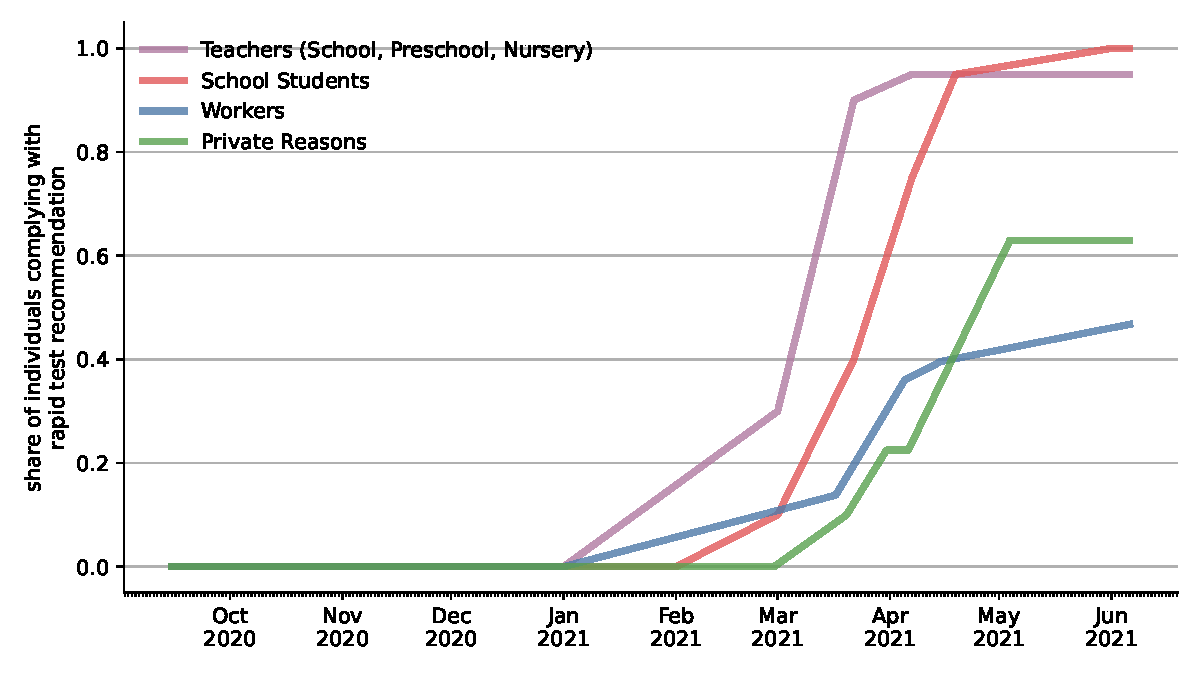
\includegraphics[width=\textwidth]{figures/results/figures/data/testing/rapid_test_demand_shares}
    \caption{\textbf{Share of Individuals Doing a Rapid Test.}}
    \floatfoot{\noindent \textit{Note:} Rapid test demand can be triggered by individuals
    planning to have education contacts, work contacts, developing symptoms without
    access to a PCR test, having a household member with a positive test or symptoms. In
    each case whether a rapid test is done depends on how long it has been since the
    individual's last rapid test and her individual compliance parameters. As an example,
    take a worker in May. In that time workers are encouraged to test themselves twice
    weekly but there is no general requirement to test themselves. If the worker has not
    done a test within the last four days in our model she will demand a test if her
    (time-constant) compliance parameter belongs to the upper 60\% in the population.}
    \label{fig:rapid_test_demand}
\end{figure}


\begin{figure}[ht]
    \centering
    \caption{Share of Individuals With Rapid Tests}
    \label{fig:share_ever_rapid_test}
    \begin{subfigure}{.55\textwidth}
        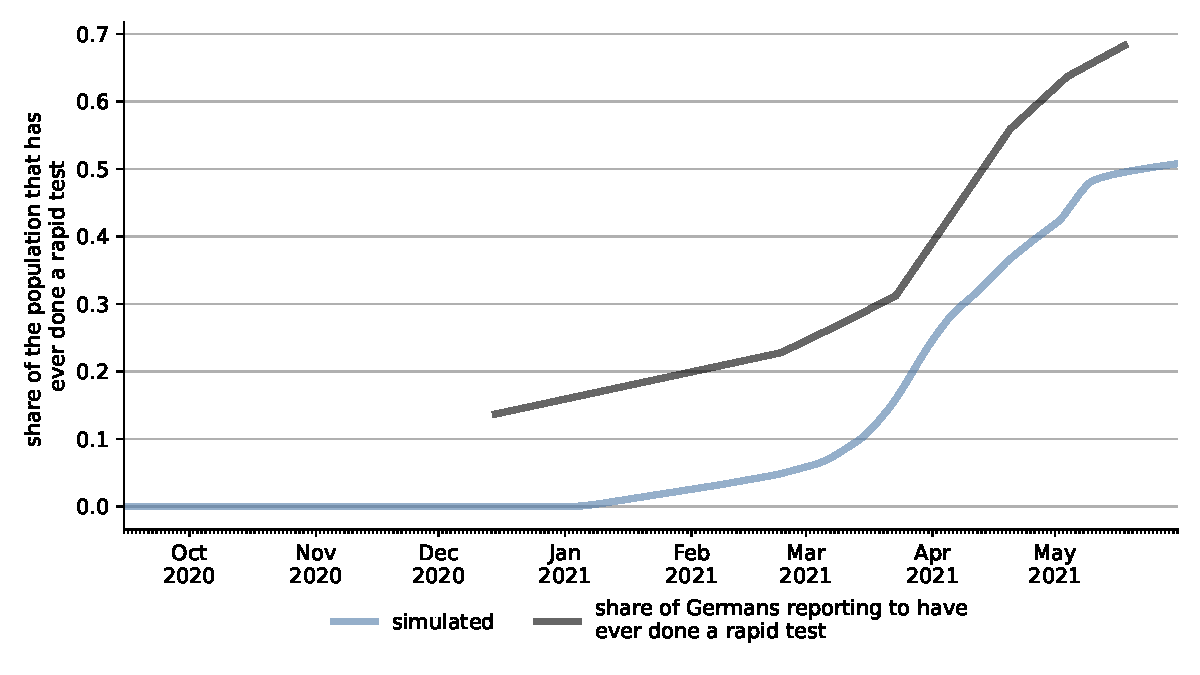
\includegraphics[width=0.9 \textwidth]{figures/results/figures/scenario_comparisons/combined_fit/full_share_ever_rapid_test}
        \caption{Share of Individuals That Have Ever Done a Rapid Test}
    \end{subfigure}%
    \begin{subfigure}{.55\textwidth}
        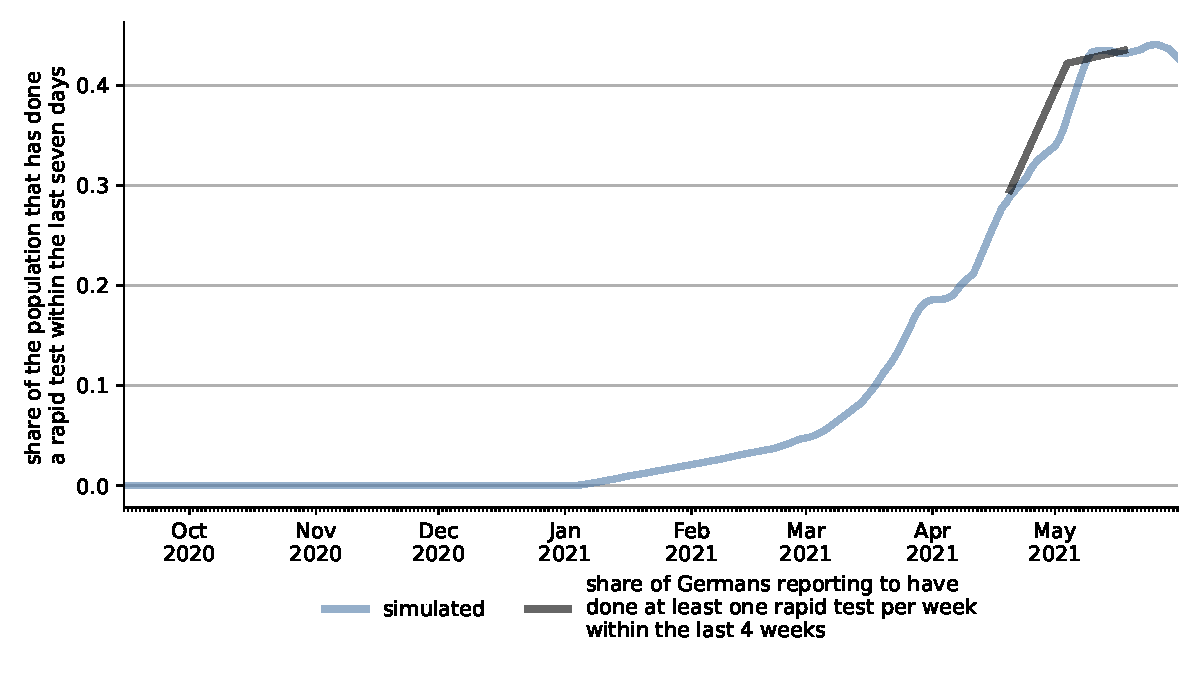
\includegraphics[width=0.9 \textwidth]{figures/results/figures/scenario_comparisons/combined_fit/full_share_rapid_test_in_last_week}
        \caption{Share of Individuals Having Done a Rapid Test in the Last Week}
    \end{subfigure}
    \label{fig:share_rapid_test_last_week}
    \floatfoot{\noindent \textit{Note:} The figure compares the share of individuals who
        have ever done a rapid test or done a rapid test within the last week in our
        simulations to the shares reported in the
        \href{https://projekte.uni-erfurt.de/cosmo2020/web/topic/wissen-verhalten/80-schnelltests/}{COVID-19
        Snapshot Monitoring Survey}. The left panel compares the share of individuals who
        have ever done a rapid test. The right panel compares the share of individuals
        who have done a rapid test within the last seven days in our simulation compared
        to the share reporting to have done at least weekly rapid tests in the last four
        weeks in the COSMO survey. Overall our calibration of rapid tests are slightly
        conservative. The overall share is below that in the study. We fit the share of
        weekly tests quite exactly. However, the study only covers adults while our share
        also includes children who are tested very regularly when attending school.}
\end{figure}

 \comment[id=K]{J: Explain that we don't fit the share ever tested that well because our rapid test compliance is completely fixed. }

\FloatBarrier

\subsection{Share of Detected Cases}
\label{subsec:data_share_known_cases}

One important feature of our model is that we distinguish between undetected and detected
cases and that we model which cases are detected and which are not (see
Section~\ref{sub:testing} for a detailed description for how we model both rapid and PCR
tests). For our model it is important to have an estimate for the share of cases that is
detected in the absence of rapid tests ($\psi_t$). For this we rely on the
\cite[Dunkelzifferradar Project][]{Dunkelzifferradar2020} which uses estimates of the
case fatality rate to estimate the number of total cases given the number of CoViD-19
deaths which are assumed to be perfectly observable. For 2020, we follow the reported
share of detected cases quite closely. One exception is the phase of November 2020 where
we interpolate to maintain monotonicity during the fall as there was no reason why the
share of detected cases should have risen in that time\footnote{The testing policy
changed in November \citep{RKI2020a}. However, this only moved the rare PCR tests more
towards vulnerable groups.}

% After Christmas 2020
Since vaccinations started after Christmas 2020 and these were predominantly given to
nursing homes in the beginning and other vulnerable groups in spring, we expect the
relationship between deaths and the number of total infections to change rapidly in 2021.
This is why we stop using the share of detected cases estimated by the Dunkelzifferradar
after Christmas. Instead, we assume that the share of detected cases would have stayed
the same in the absence of rapid tests. Thus, we also achieve in our model an increase in
the share of detected cases but this is driven from inside our model through increased
rapid testing which lead follow-up PCR tests when they are positive (see
Section~\ref{subsec:results_share_known_cases} and \ref{sub:testing}).

% Christmas and Easter
Lastly, we model reductions in the share of detected cases due to the two major holidays in our
simulation period, Christmas and Easter. During both holidays many laboratories did not
process tests and most physicians' offices were closed, leading to less PCR tests and
short and large drops in the share of known cases. The resulting share of detected cases
in the absence of rapid tests is shown in Figure~\ref{fig:share_known_cases_data} and
was estimated to fit the data.

\begin{figure}[ht]
  \centering
  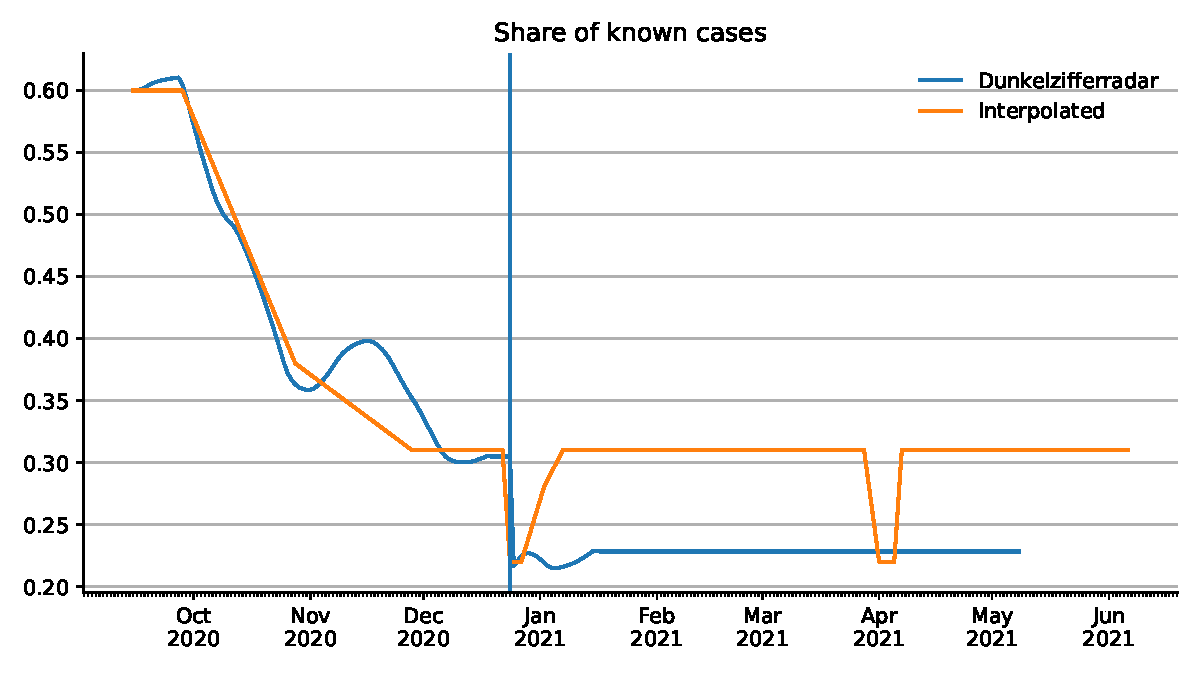
\includegraphics[width=0.5\textwidth]{figures/results/figures/data/testing/assumed_overall_share_known_cases}
  \caption{Share of Detected Cases in the Absence of Rapid Tests}
  \label{fig:share_known_cases_data}
  \floatfoot{\noindent \textit{Note:} The figure shows the share of cases that is
  reported as an official case via PCR confirmation. We use the overall share of known
  cases that was estimated through the case fatality ratio by the \cite[Dunkelzifferradar
  Project][]{Dunkelzifferradar2020} for all of 2020 and then assume it to be constant as
  vaccinations of the elderly strongly affect the case fatality rate which the project
  does not account for. Starting in 2021 in addition to the overall numbers of detected
  cases through symptoms and a random component, cases are also detected through
  confirmation of positive rapid tests which happens endogenously inside the model. For
  the public holidays of Christmas and Easter we lower the share of detected cases as
  fewer PCR tests are available during public holidays. See
  Figure~\ref{fig:share_known_cases_by_age_group} for how the share of detected cases
  develops in our model for each age group}.
\end{figure}

\FloatBarrier

